\documentclass[main.tex]{subfiles}
\begin{document}


% BTK: Waurm wurde so evaluiert ? Damit es wissenschaftlich ist.  
\chapter{Evaluation}

Ob ein Framework oder ein \gls{osre} performant ist, kann kaum aus der Literatur entnommen werden. Auch Benchmarks stossen dabei an ihre Grenzen wenn es darum geht vergleiche zwischen Frameworks zu machen die je nach Einsetzungsgebiet verschiedene Stärken oder Schwächen ausweisen können. Dadurch kann eine objektive Aussage zwar wahr sein,  ist womöglich aber für das eigene Projekt nicht aussreichend oder sogar falsch. Es wurde entschieden einen eigenen Prototypen zu erstellen der  in dieser Arbeit  zu evaluieren gilt. 

Für die Evaluation wurde bestimmt dass  die Prototypen abwechslungsweise auf die PaaS zu deployen um diese separat von einander analysieren zu können. Gegen die deployten Prototypen wurden automatische Lasttest durchgeführt. Da die Performancemessungen mehrmals zu erheben waren  wurde ein Testplan vorgängig erstellt. Damit konnte die Test vorgängig konfiguriert und automatisiert durchgeführt werden. Die wichtigsten Performancemessungen wurden einerseits mit dem Testtool JMeter genereiert und andererseits mithilfe der Logs auf der PaaS erhoben. Dank der Konsolidierung dieser Dateien konnten Rückschlüsse auf die Performance gezogen werden.

Die Evaluation teilt sich in drei Teile auf (siehe Abbildung \ref{figure:evaluationsAblauf}) diese Teile werden in den folgenden Kapitel näher erläutert. 

\begin{figure}[h]
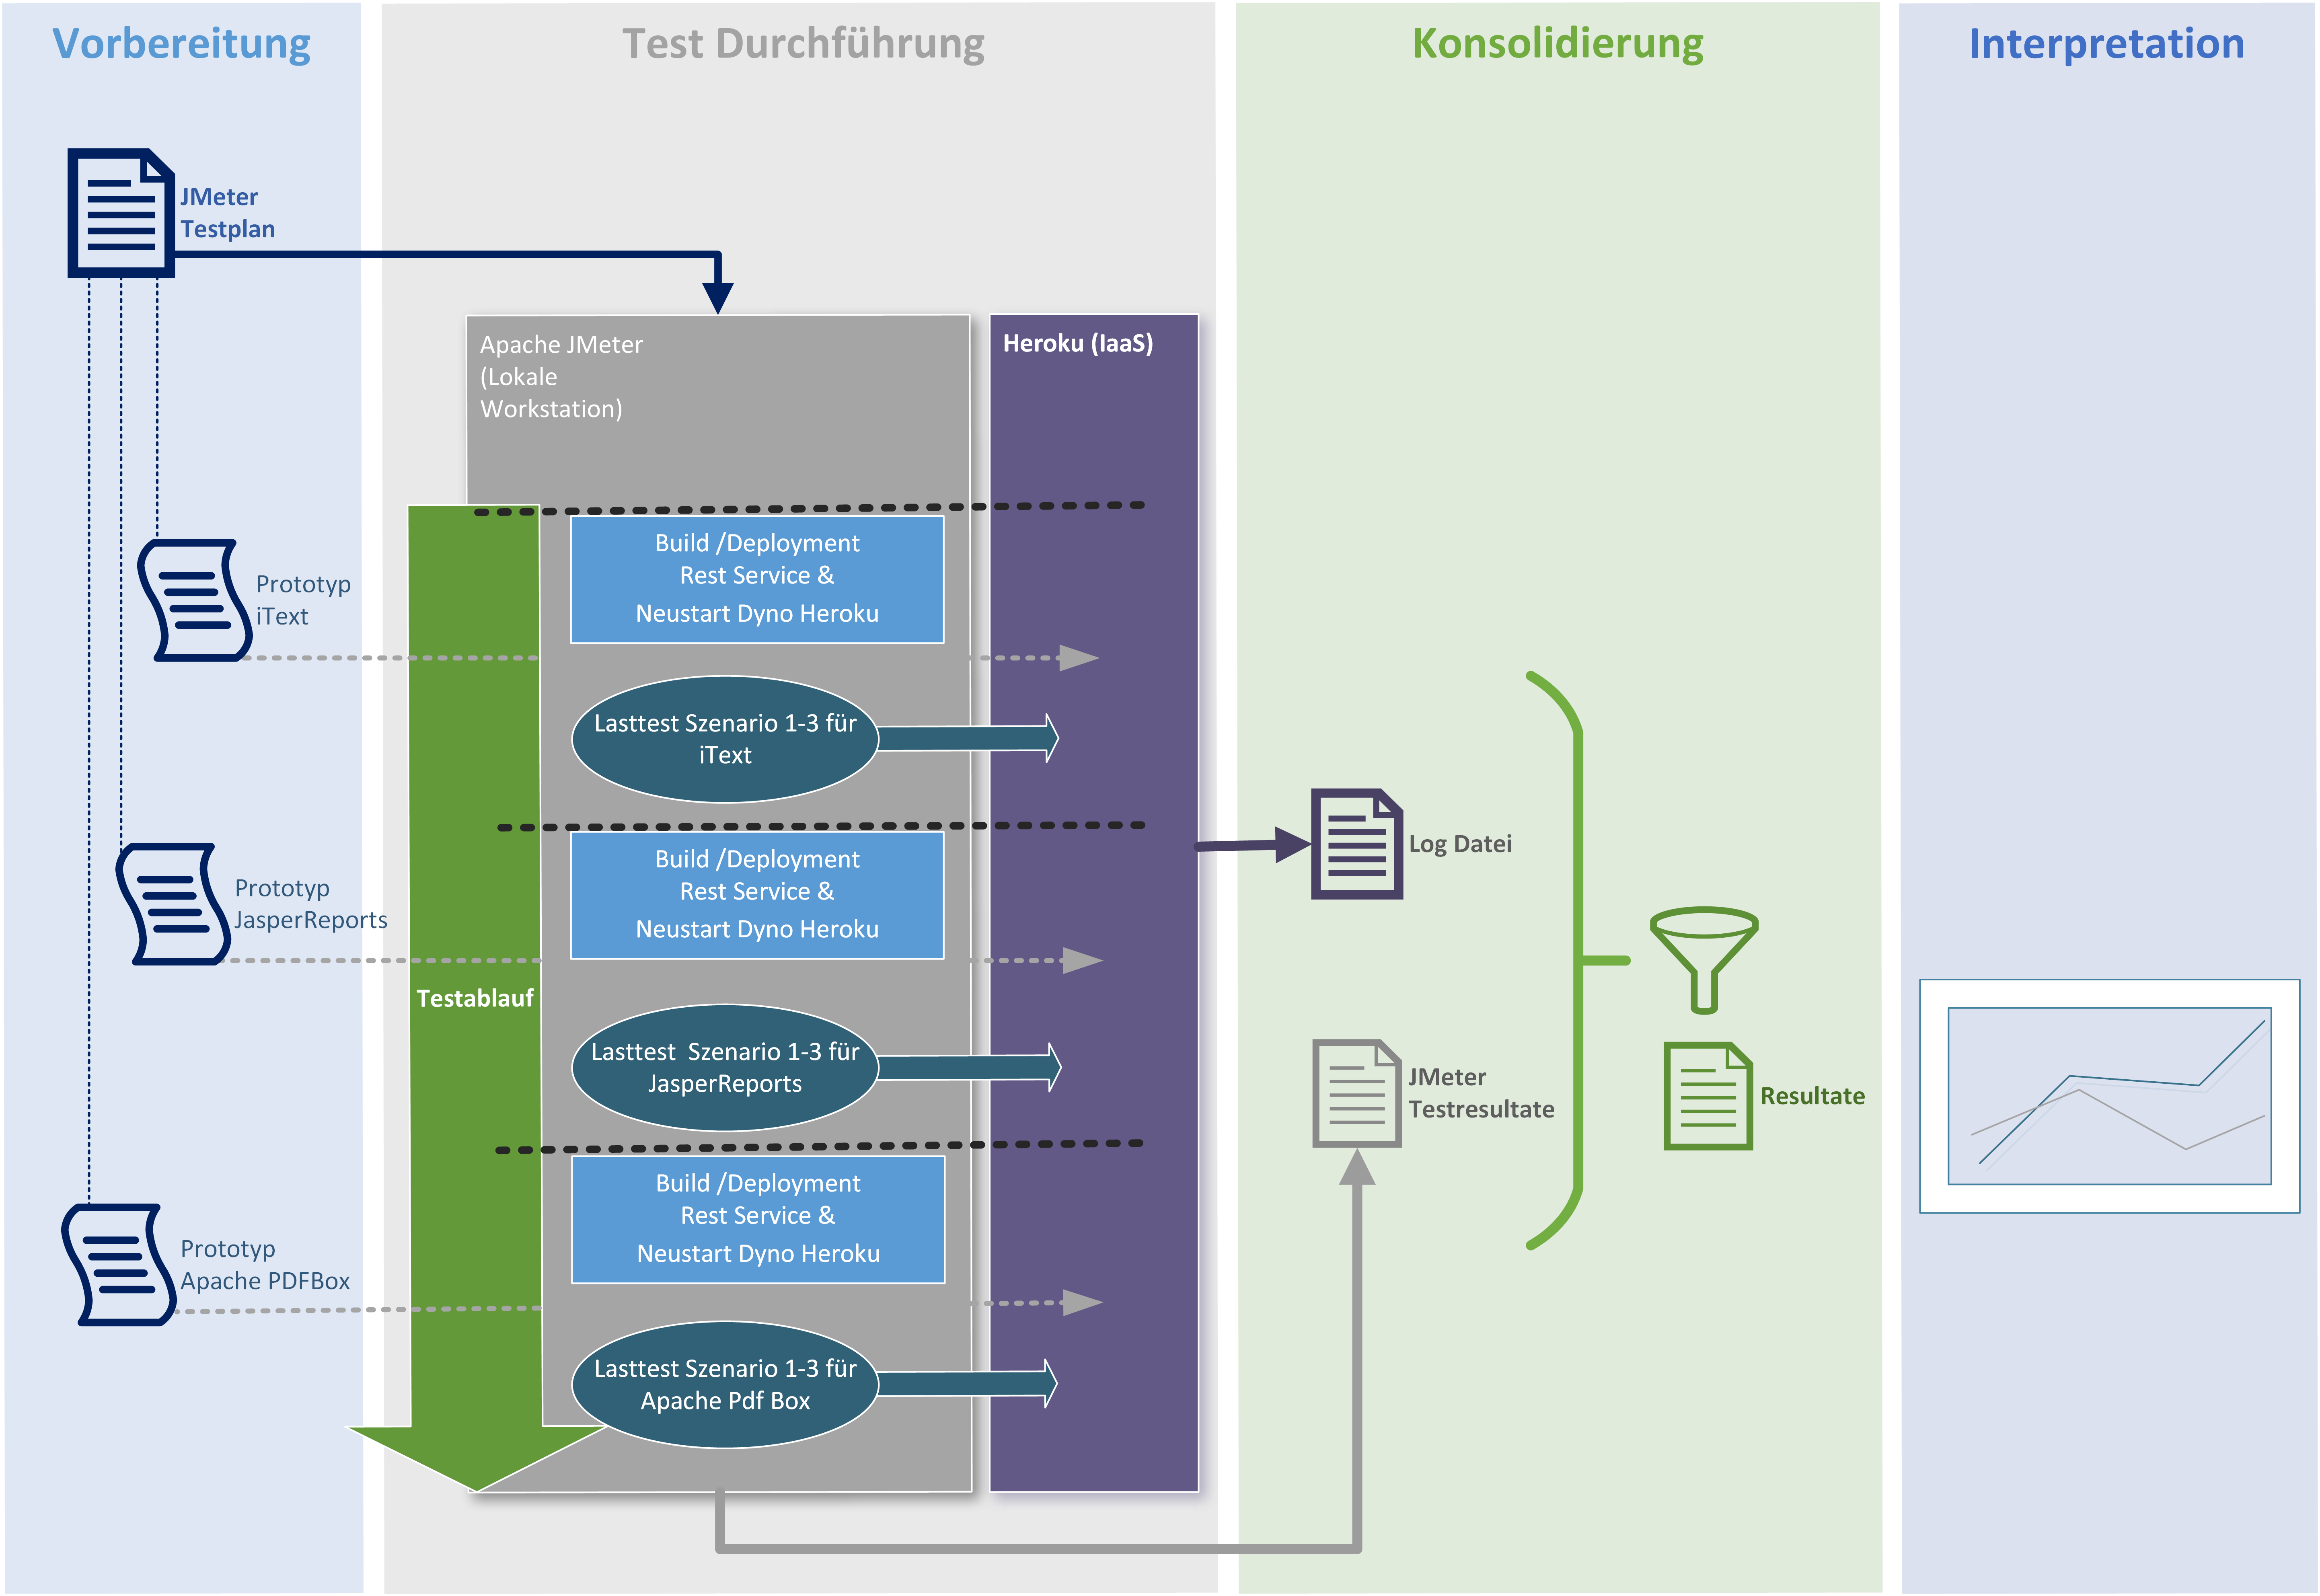
\includegraphics[width=\textwidth]{mainpart/3_methodik_evaluation_img/Testablauf.png}
 \caption{Evaluationsablauf}
 \label{figure:evaluationsAblauf}
\end{figure}


\section{Vorbereitung}
In der Phase Vorbereitung geht es darum die Prototypen zu erstellen sowie den Testplan zu definieren. Die Details zur Erstellung der Prototypen werden später erläutert.

\subsection{Testplan}
Im Testplan müssen verschiedene Parameter definiert werden, wie diese gewählt werden bestimmt der Anwendungsfall der hier behandelt wird.

\textbf{Last-Strategie}\newline
Eine Nutzergruppe kann auf ein produktives System verschiedene Last-Muster generieren dabei gelingt es den Usern durch den Ansturm auch grosse Rechenzentren Lahmzulegen. Ob alle User gleichzeitig wie z.B. beim Vorverkauf von Konzertkarten an den gebotenen Service anmelden oder gestaffelt, ist für ein System durchaus wichtig, denn je nach Service kann dieser sich mit der Anzahl Anfragen an den neuen Umständen anpassen und  horizontal Skalieren, also die Last auf viele verschiedene Server verteilen. 

\textbf{Ramp-Up}\newline
Bei den durchgeführten Lasttest wurde die Infrastruktur nicht skaliert, dennoch wurde eine Ramp-Up von 10 Sekunden definiert, was bedeutet dass die gesamte Menge der virtuellen User nach 10 Sekunden auf dem System aktiv Last erzeugen. Dieses Szenario wurde gewählt da sich in der Praxis fast nie Systeme gleich vollständig ausgelastet werden. 

Da es in diesen Experimenten darum geht verschiedene Anwendungen und deren Frameworks zu evaluieren wurde eine fixe Anzahl User definiert die sich über 10 Sekunden hinweg alle zuschalten und  10 Minuten lang auf dem System 'arbeiten', somit variieren sich diese über den Test hin weg nicht mehr. Diese Strategie wurde gewählt da es einfacher ist die Messungen zu evaluieren und die Performancemessungen zuverlässiger gesammelt werden können. 

\textbf{Last}

Ein Service kann in verschiedenen Arten belasstet werden. Einserseits, was öfter vorkommt, ist das steigen der aktiven User auf dem System. Diese Last wird meist über eien Scale out der Server behoben. Was ebenfalls vorkommt ist dass die Last auf dem Service durch grössere Anfragen gefordert d.h. Requestgrössen steigen. Das kann z.B bei Services die  eine Bestandeslieferung von Einwohnern entgegen nimmt. Diese Anfrage nimmt meist Jährlich zu oder auch möglich ist das grössere Gemeinden als Kunden dazu gezählt werden dürfen.  

In dieser Arbeit wurden die beiden Lasten im Testplan miteinbezogen. Bei den Tests wurden einerseits die virtuellen User von 20 auf 50 gesetzt und andererseits wurden die virtuellen User bei 20 belassen aber die Requestgrösse verdreifacht. D.h. die zu verarbeitenden Datensätze wurden verdreifacht nicht die Bytegrösse der Anfragen.
Diese Tests sollen Aufschluss geben wie sich die OSREs bei Lasterhöhung verhalten.

\subsection{Testplan}

Die definierten Parameter und Testpläne wurden als jmx-Datei festgehalten und für die Testdurchführung aufbereitet. 


\begin{reference}{JMeter Testplan}
Der Basisplan kann im Anhang gefunden werden oder unter: 
 \url{https://github.com/denisbittante/dinf/tree/master/loadtest/jmeter/DinfLoadTest.jmx}
 
\end{reference}



\section{Test Durchführung}


Um die Performance einzelner Implementationen testen zu können wurden eine Serie von Test erstellt, die als Lastest gegen die Services liefen. Die Lasttests spiegelten die Anforderungen an Services wieder dabei wurden verschiedenen Parameter angepasst die in der Praxis ebenfalls anzutreffen sind. Im folgenden werden diese kurz erläutert.

\subsection{JMeter}


Um die definierten Testszenarien durchzuführen wurde  das Open Source Tool Apache JMeter (v.3.3) genutzt. Das Tool unterstützt eine Reihe verschiedener Protokolle unter anderem REST was für dieses Experiment genutzt wurde. Die Testszenarien wurden im  "Non-GUI"-Mode durchgeführt, dieser dient dazu intensive Testreihen in einem CLI-Umgebung durchzuführen.
Um die Test durchzuführen wurde  folgendes Skript erstellt um die Testergebnisse mit Zeitangabe zu speichern.

\begin{lstlisting}[language=command.com]
           
@echo off
for /f "tokens=2 delims==" %%a in ('wmic OS Get localdatetime /value') do set "dt=%%a"
set "YY=%dt:~2,2%" & set "YYYY=%dt:~0,4%" & set "MM=%dt:~4,2%" & set "DD=%dt:~6,2%"
set "HH=%dt:~8,2%" & set "Min=%dt:~10,2%" & set "Sec=%dt:~12,2%"

set "datestamp=%YYYY%%MM%%DD%" & set "timestamp=%HH%%Min%%Sec%"
set "fullstamp=%YYYY%-%MM%-%DD%_%HH%-%Min%-%Sec%"

jmeter -n -t C:/sandbox/dinf/dinf/loadtest/jmeter/LoadTest-TIMED.jmx -l C:/sandbox/dinf/dinf/loadtest/jmeter/testlog-%fullstamp%.jtl

\end{lstlisting}




\begin{reference}{JMeter Ressourcen}
 Die originalesn PDFs können hier eingesehen werden: \url{https://github.com/denisbittante/dinf/tree/master/doc/results/pdf}
 
\end{reference}



\subsection{Test Szenarien}
Es wurden verschiedene Szenarien definiert die einerseits ein mögliches Anwendungsbereich von OSRE abbilden könnten andererseits sich an die Speziellen Implemenatation der OSRE richten. Als Beispiel verfügt Apache PDF Box nicht über eine Integrierte Schnittstellen um Tabellen zu implementieren. Im folgenden werden diese Szenarien detaillierter vorgestellt.  


\begin{reference}{PDF Resultate}
 Die originalen PDFs können auf GitHub oder im Anhang nachgeschlagen werden: \url{https://github.com/denisbittante/dinf/tree/master/doc/results/pdf}
 
\end{reference}

\subsubsection{Szenario 1}


\fbox{
\includegraphics[scale=0.23]{mainpart/3_methodik_evaluation_img/itextSZ1.pdf}}
\fbox{
\includegraphics[scale=0.23]{mainpart/3_methodik_evaluation_img/jasperSZ1.pdf}}
\fbox{
\includegraphics[scale=0.23]{mainpart/3_methodik_evaluation_img/itextSZ1.pdf}}
Wie in Problembeschreibung erwähnt wurde ein reale Anforderung skziert. Aufgrund derer wird ein PDF Erarbeitet die eine erwartet länge von 3-4 Seiten lang ist. Der Prototyp soll mit der beschriebenen Rahmenbedingung ausgetestet werden, wobei die beschriebenen 270'000 Reports auch in wenigen Minuten generiert werden sollen, da nicht davon ausgegangen wird das diese Reports im Verlauf von wenigen Tagen z.B. Anfangs Monat erstellt werden. Da es sich in diesem Beispiel um Programme handeln die einen Monat umfassen werden pro Monat ein Programm erstellt und versendet oder ausgedruckt. 
\subsubsection{Szenario 2}

\fbox{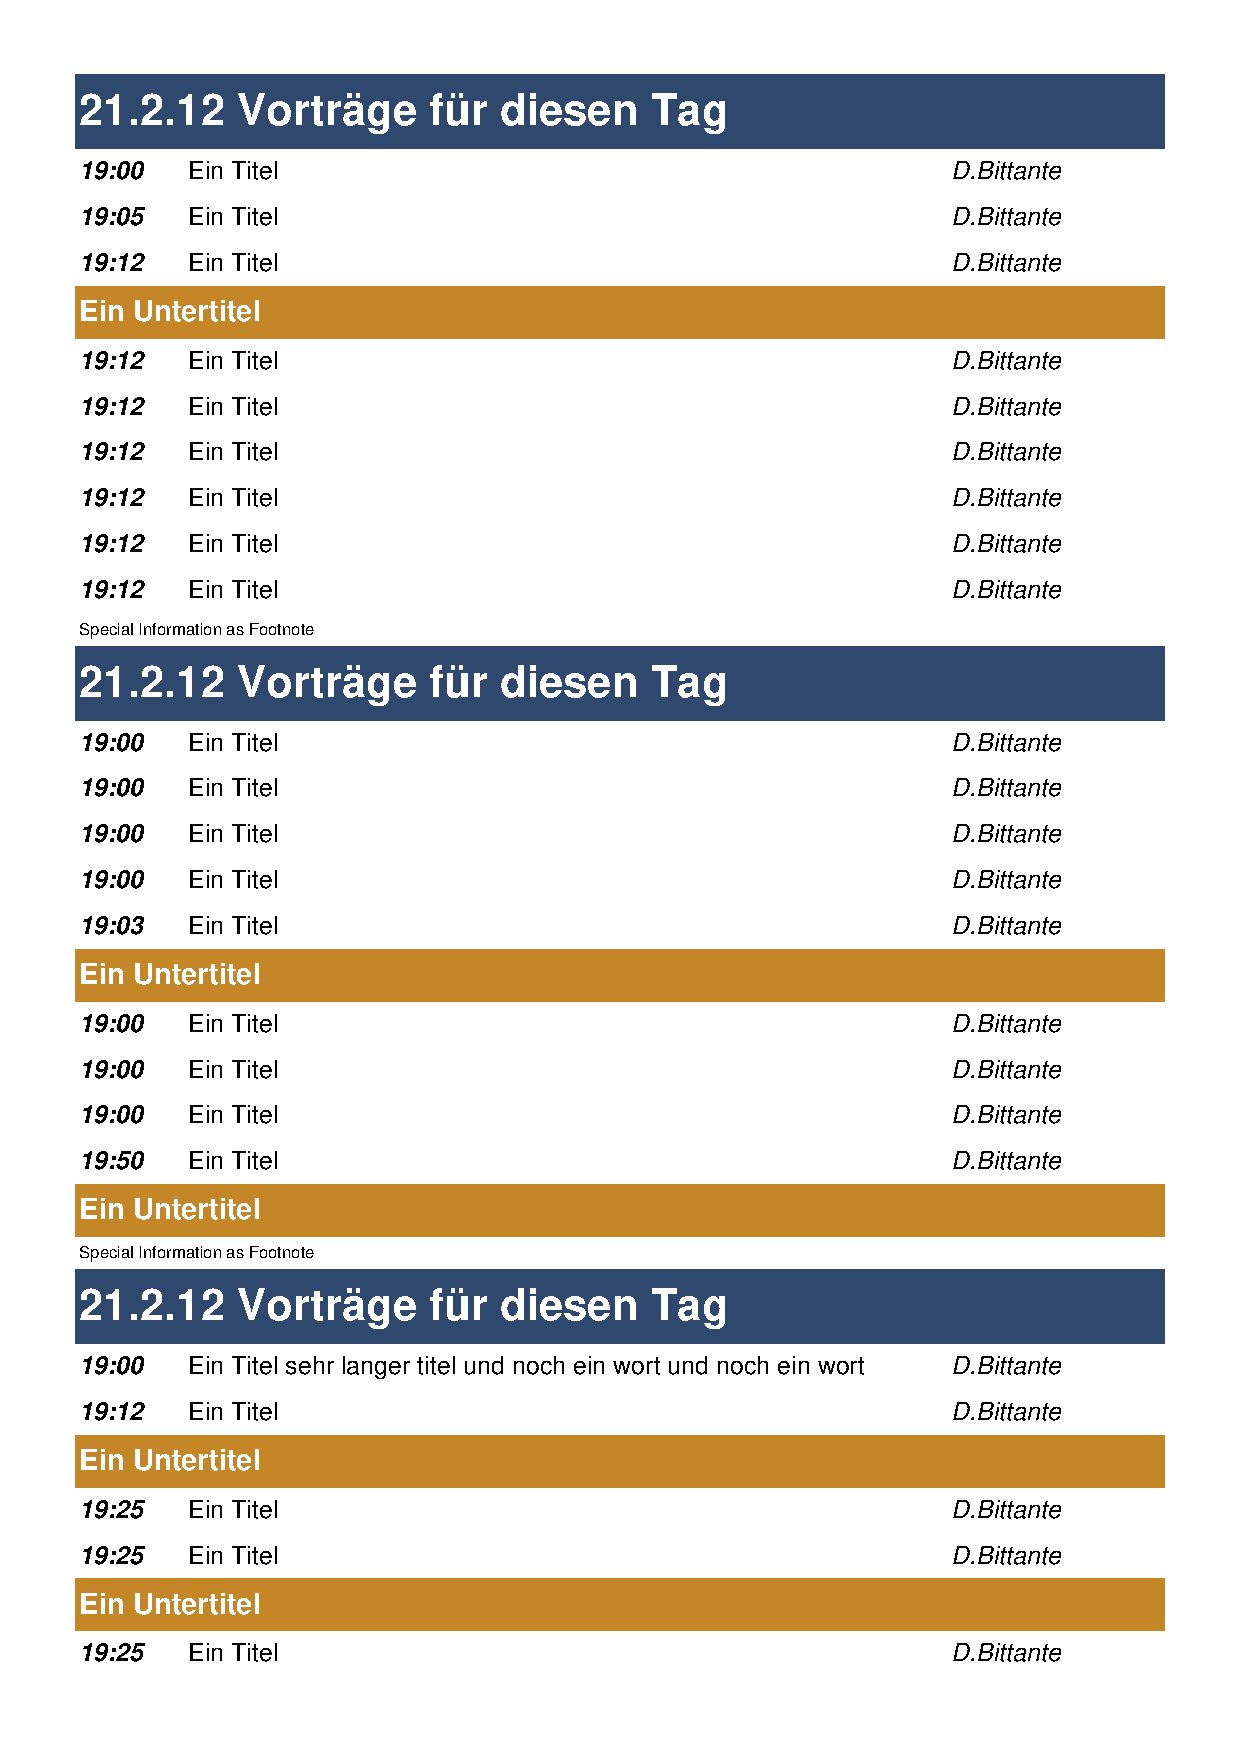
\includegraphics[scale=0.23]{mainpart/3_methodik_evaluation_img/itextSZ2.pdf}}
\fbox{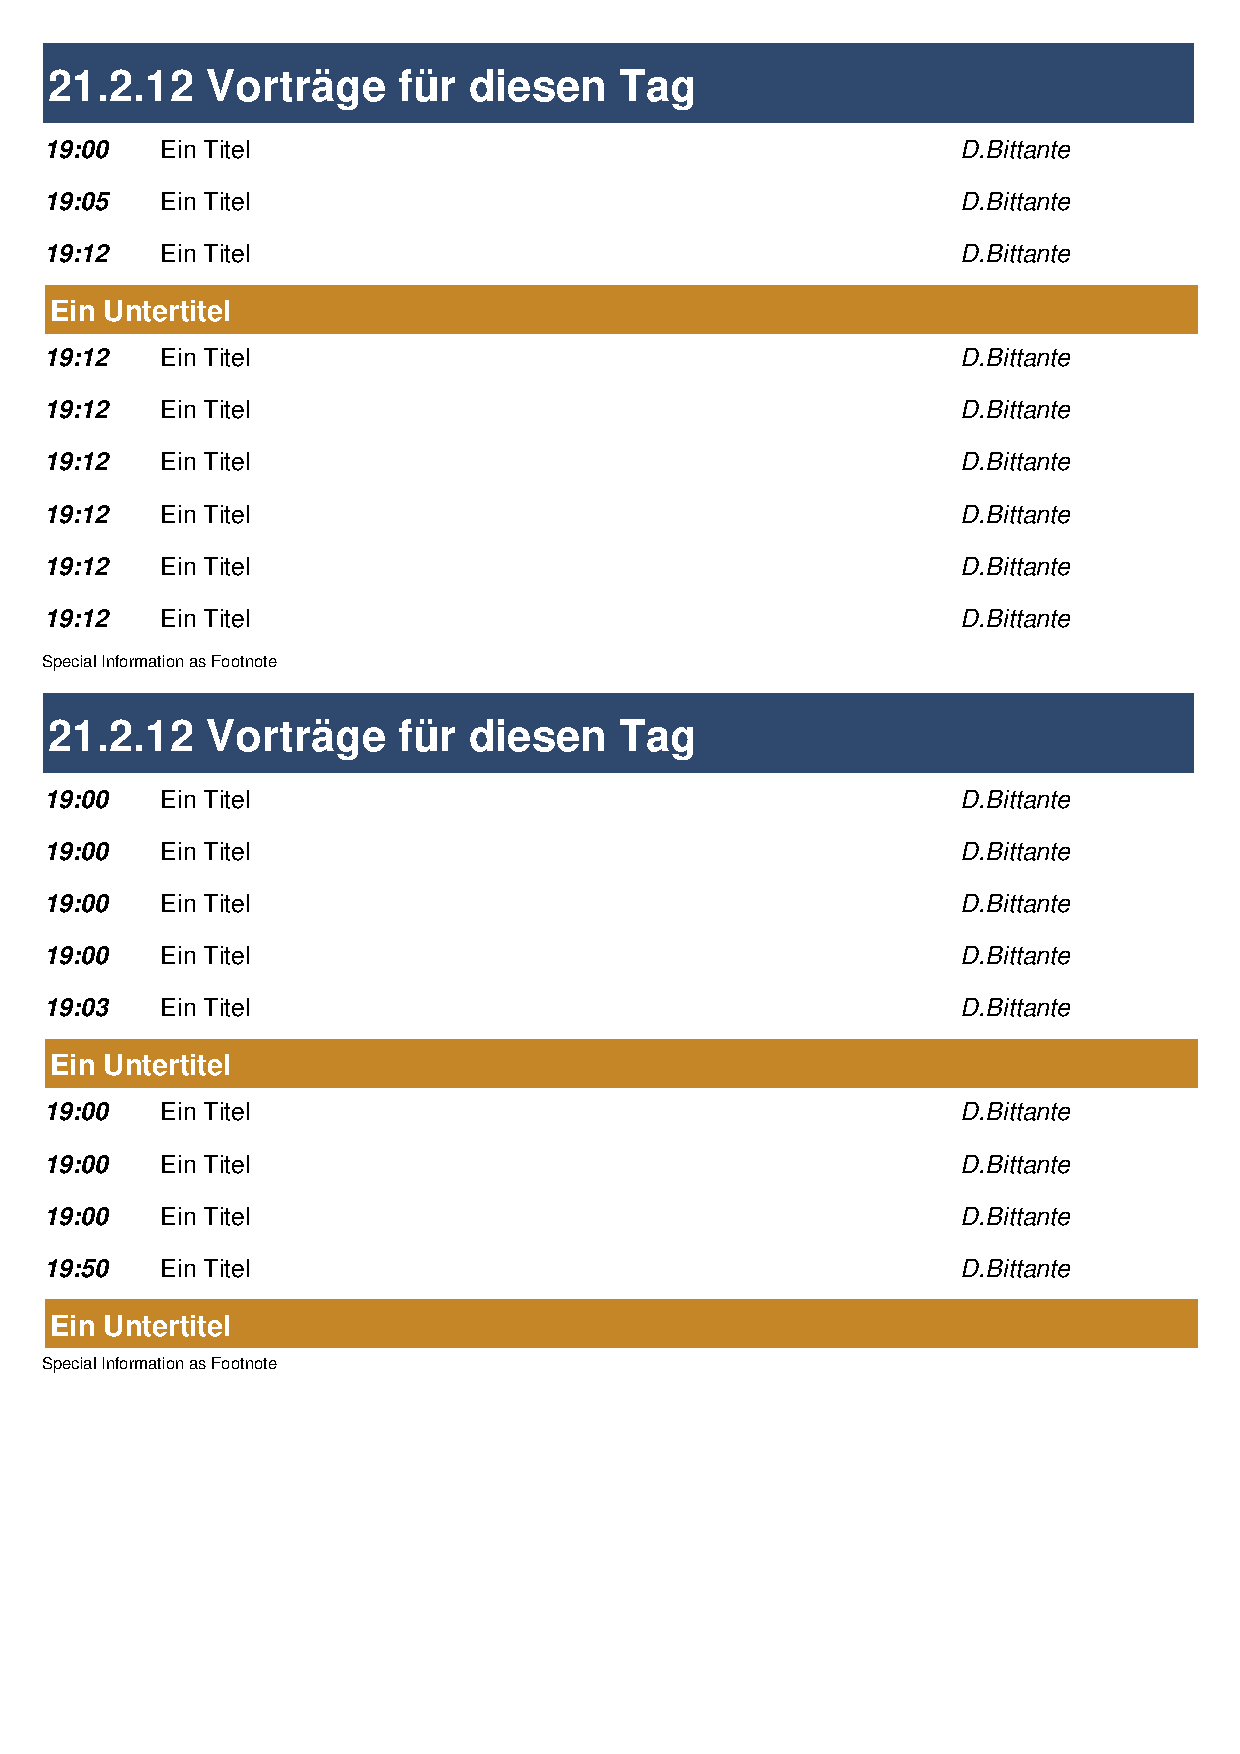
\includegraphics[scale=0.23]{mainpart/3_methodik_evaluation_img/jasperSZ2.pdf}}
\fbox{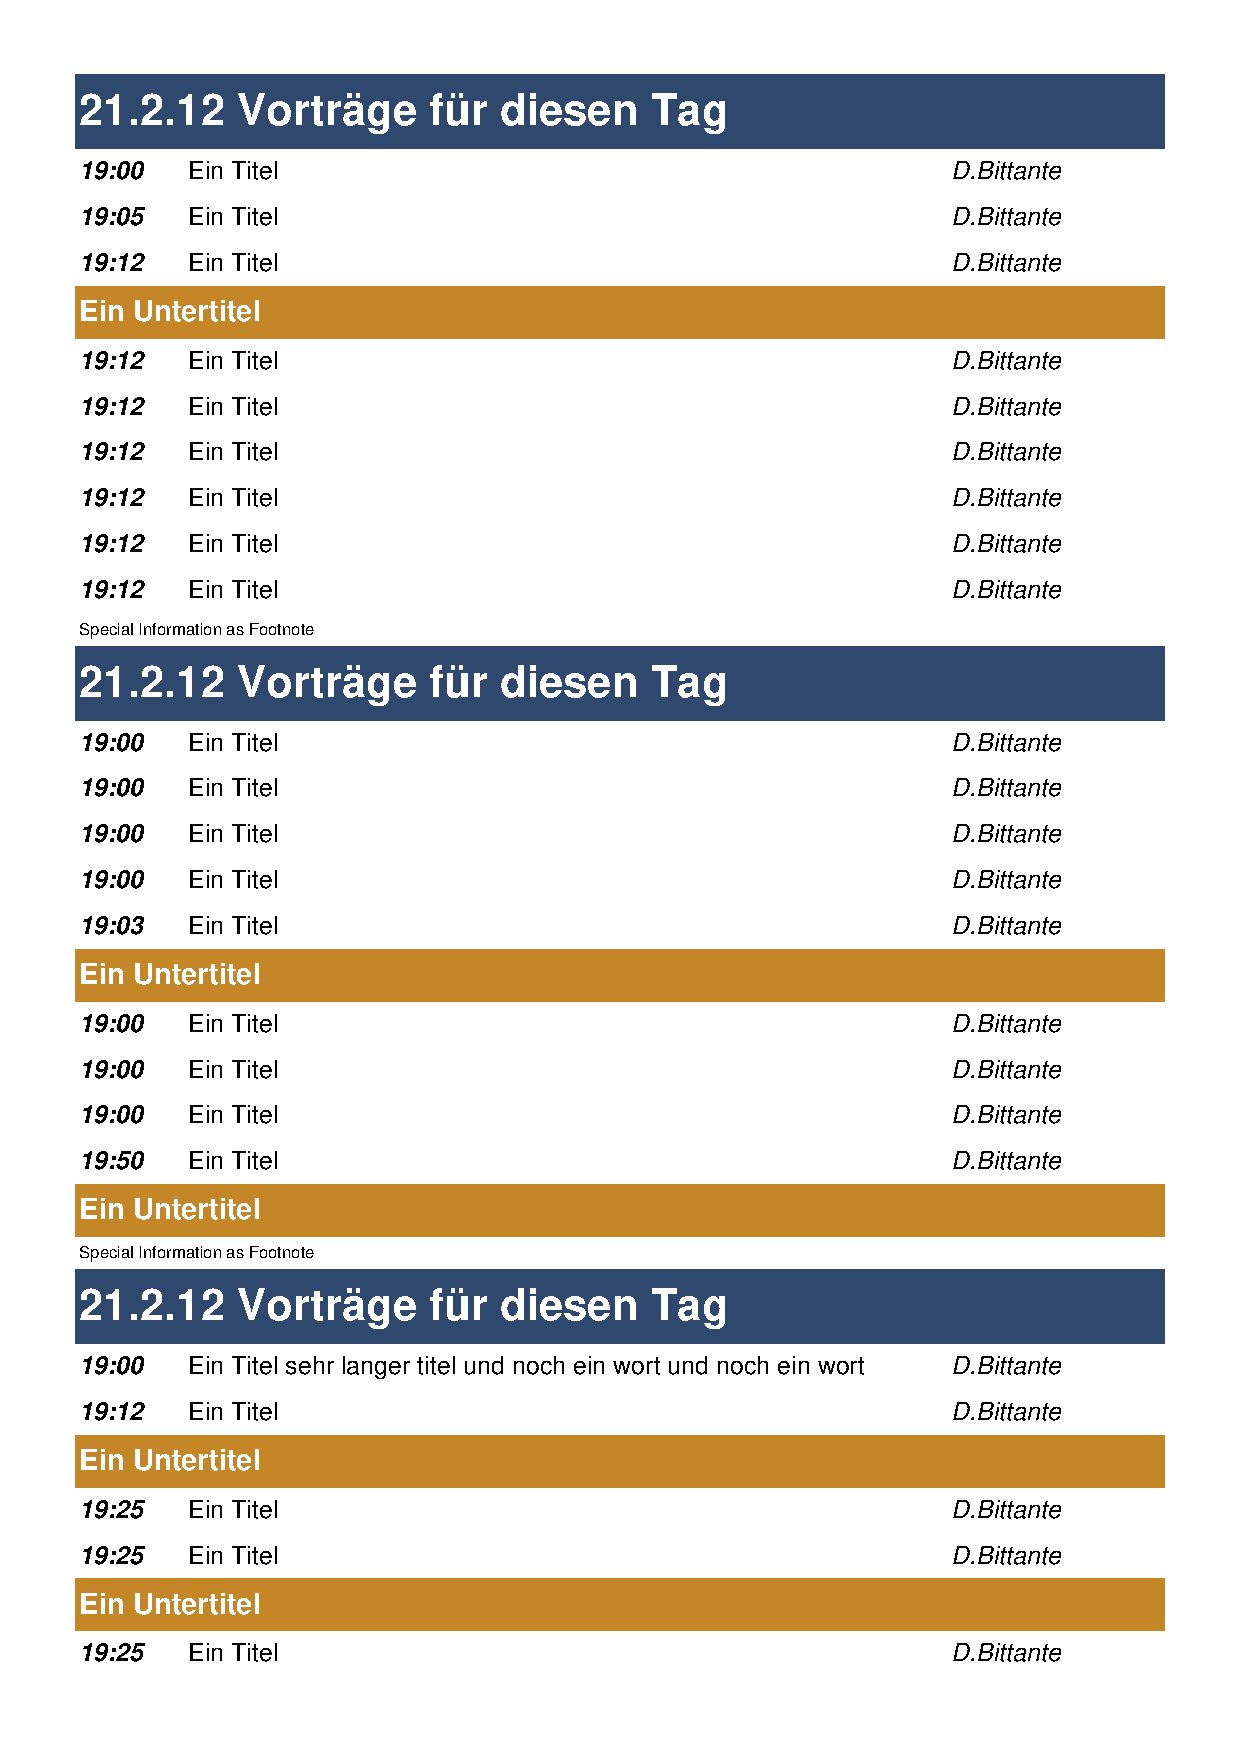
\includegraphics[scale=0.23]{mainpart/3_methodik_evaluation_img/itextSZ2.pdf}}

In diesem Anwendungsfall gilt es zu prüfen wie eine OSRE mit komplexem Seitenaufbau zu recht kommt und wie sich das auf die Performance auswirkt und vor allem wie die Ressourcen dabei genutzt werden . Dabei soll der Seitenaufbau kompliziert (d.h. mit Kopf- und Fusszeilen, definierten Rändern und Mehrspaltig) sowie die Datenmengen sehr umfangreich ausfallen  der Länge eines PDFs soll etwa 30 - 40 Seiten betragen. 

\subsubsection{Szenario 3}

\fbox{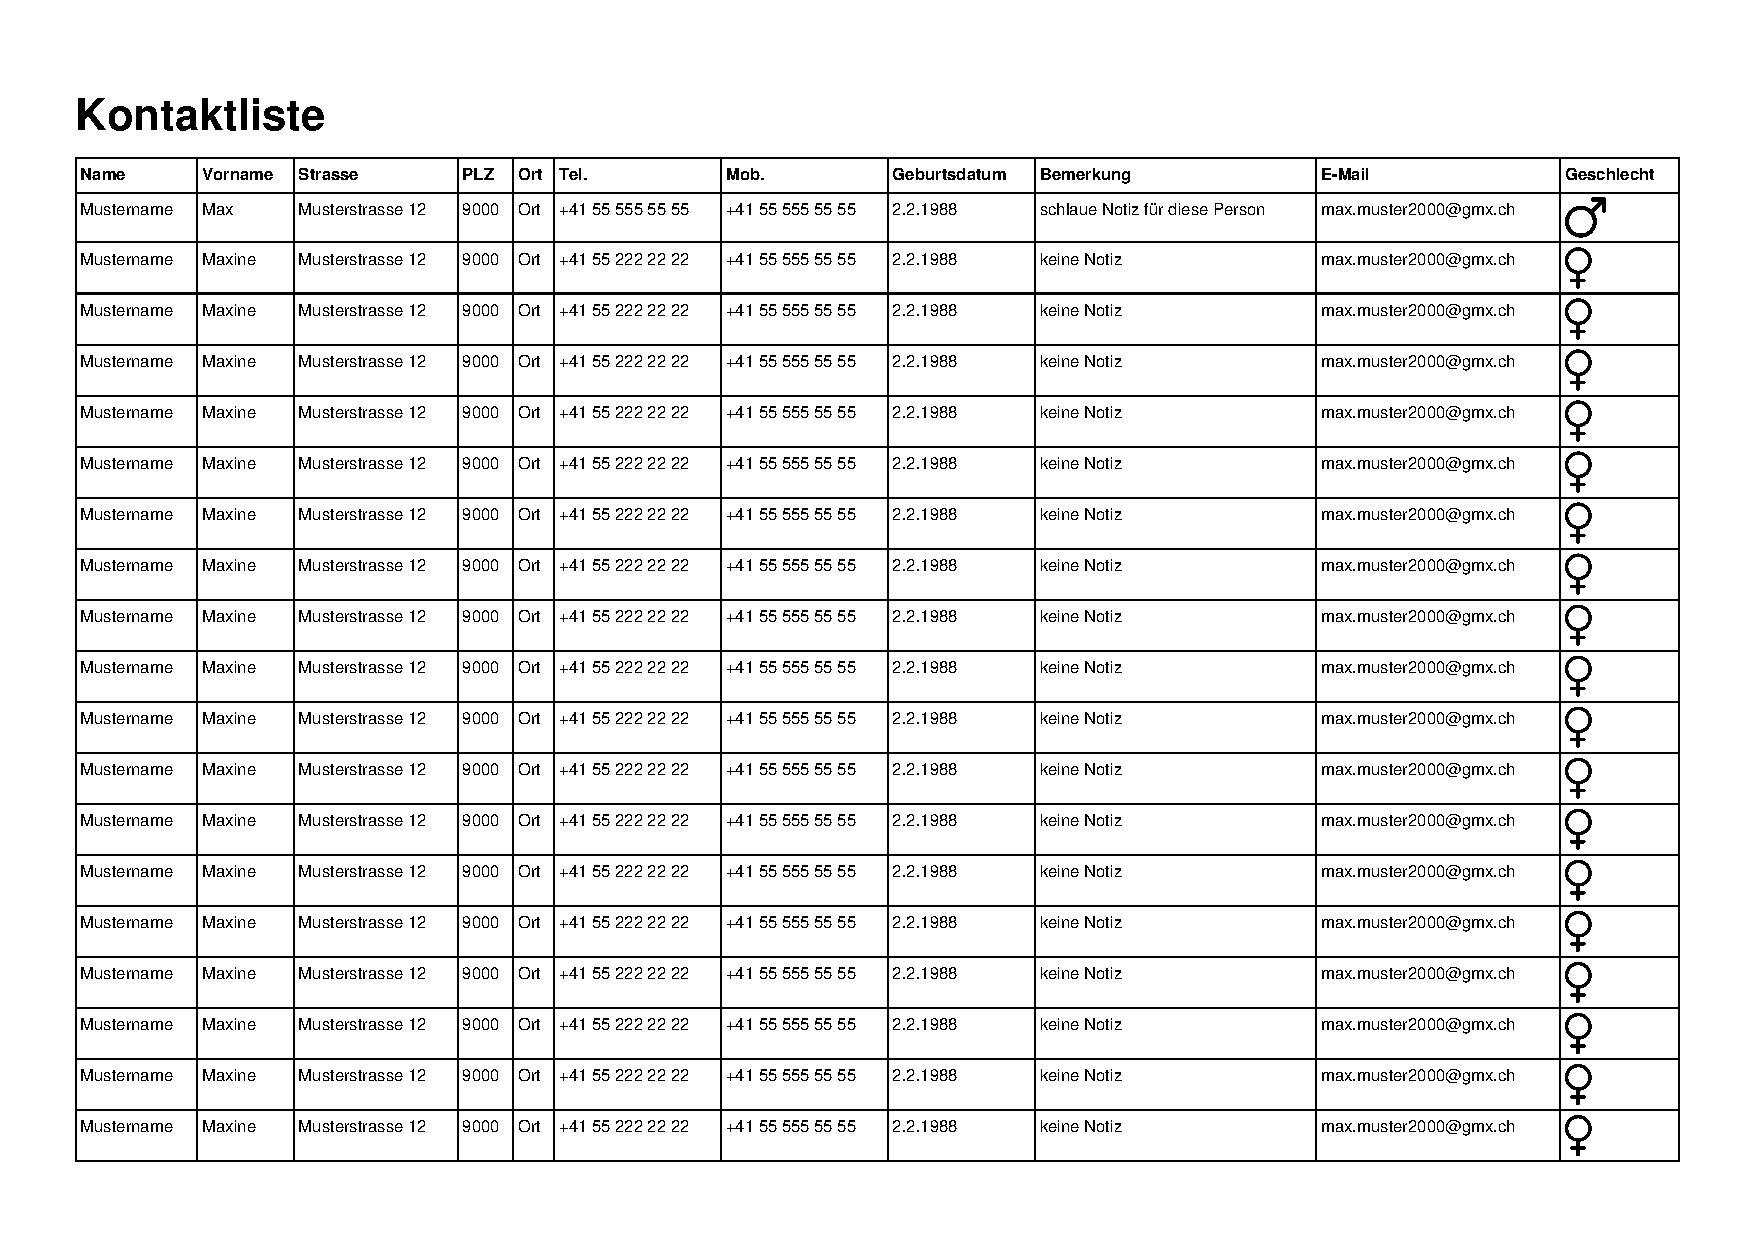
\includegraphics[scale=0.16]{mainpart/3_methodik_evaluation_img/itextSZ3.pdf}}
\fbox{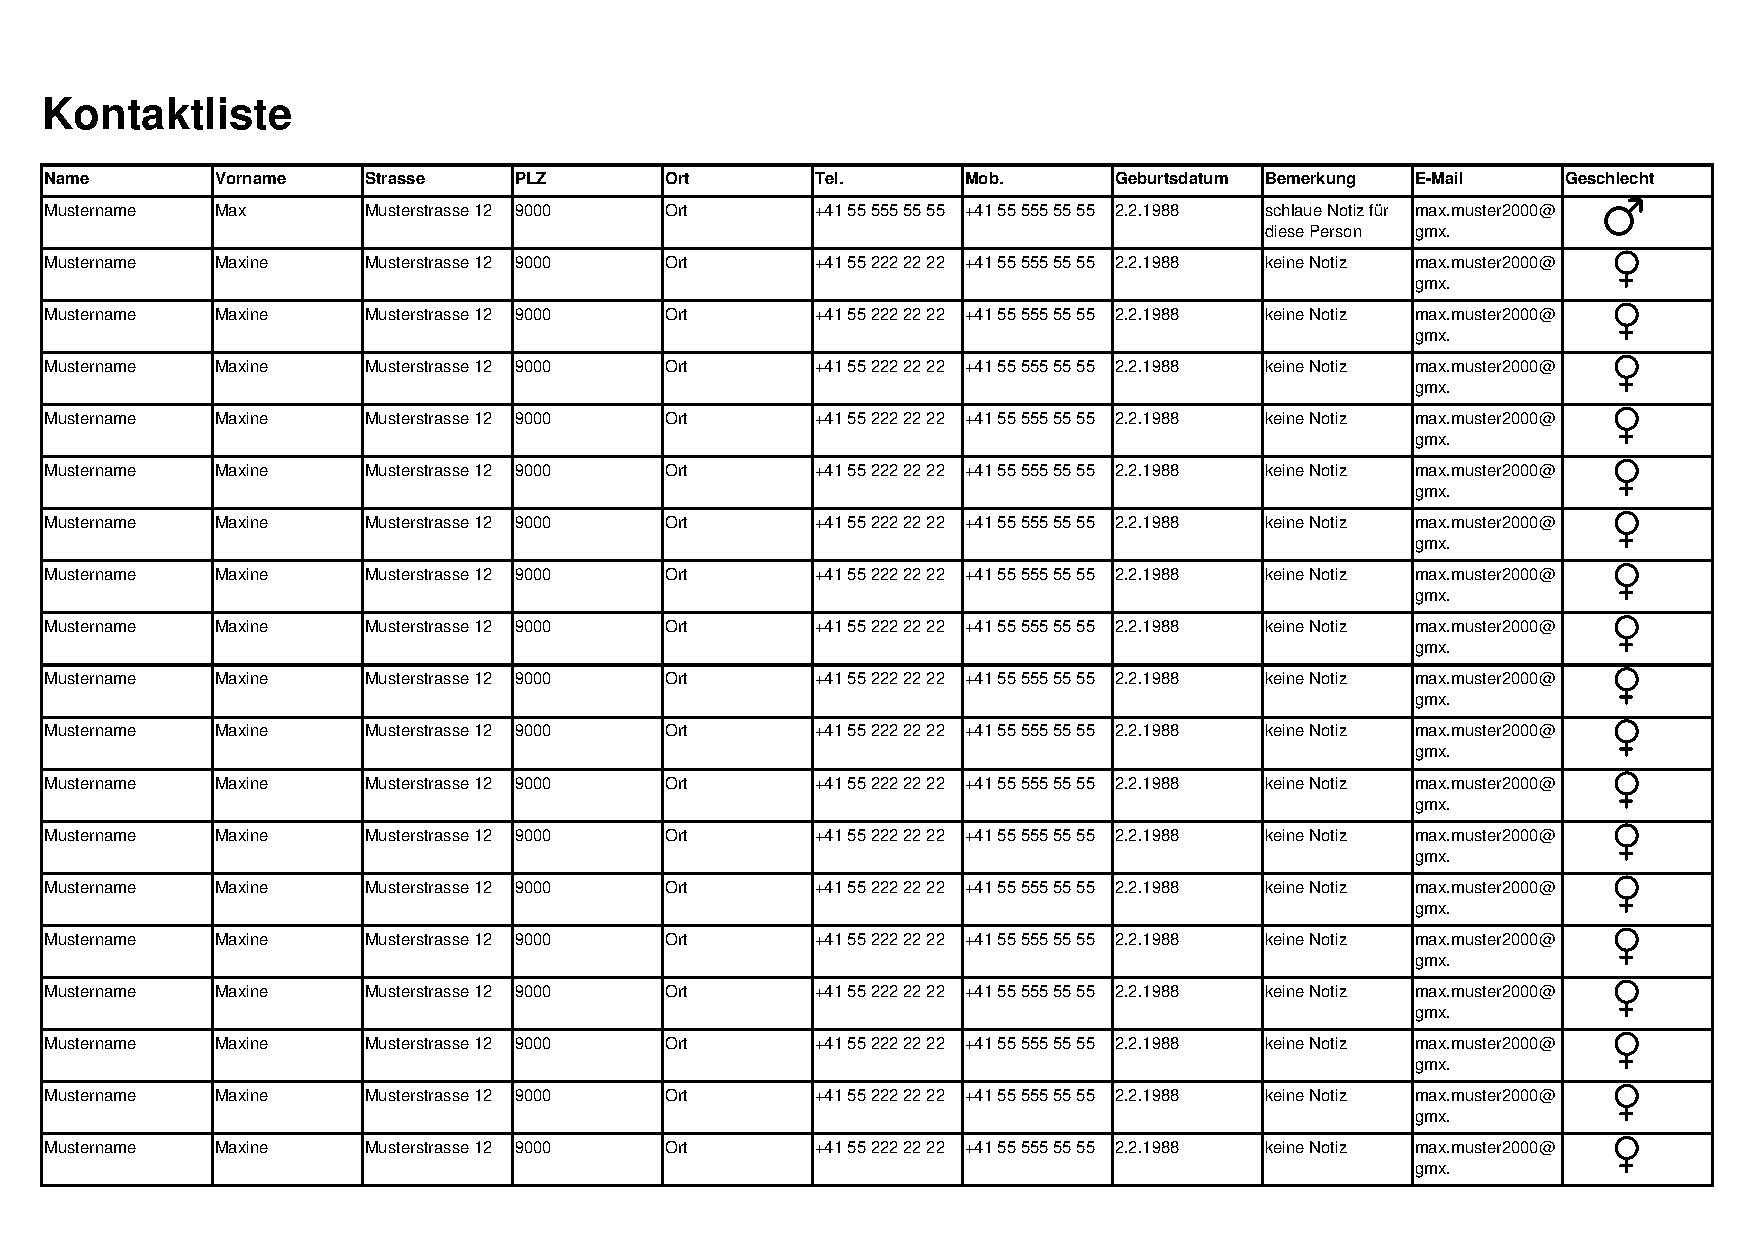
\includegraphics[scale=0.16]{mainpart/3_methodik_evaluation_img/jasperSZ3.pdf}}
\fbox{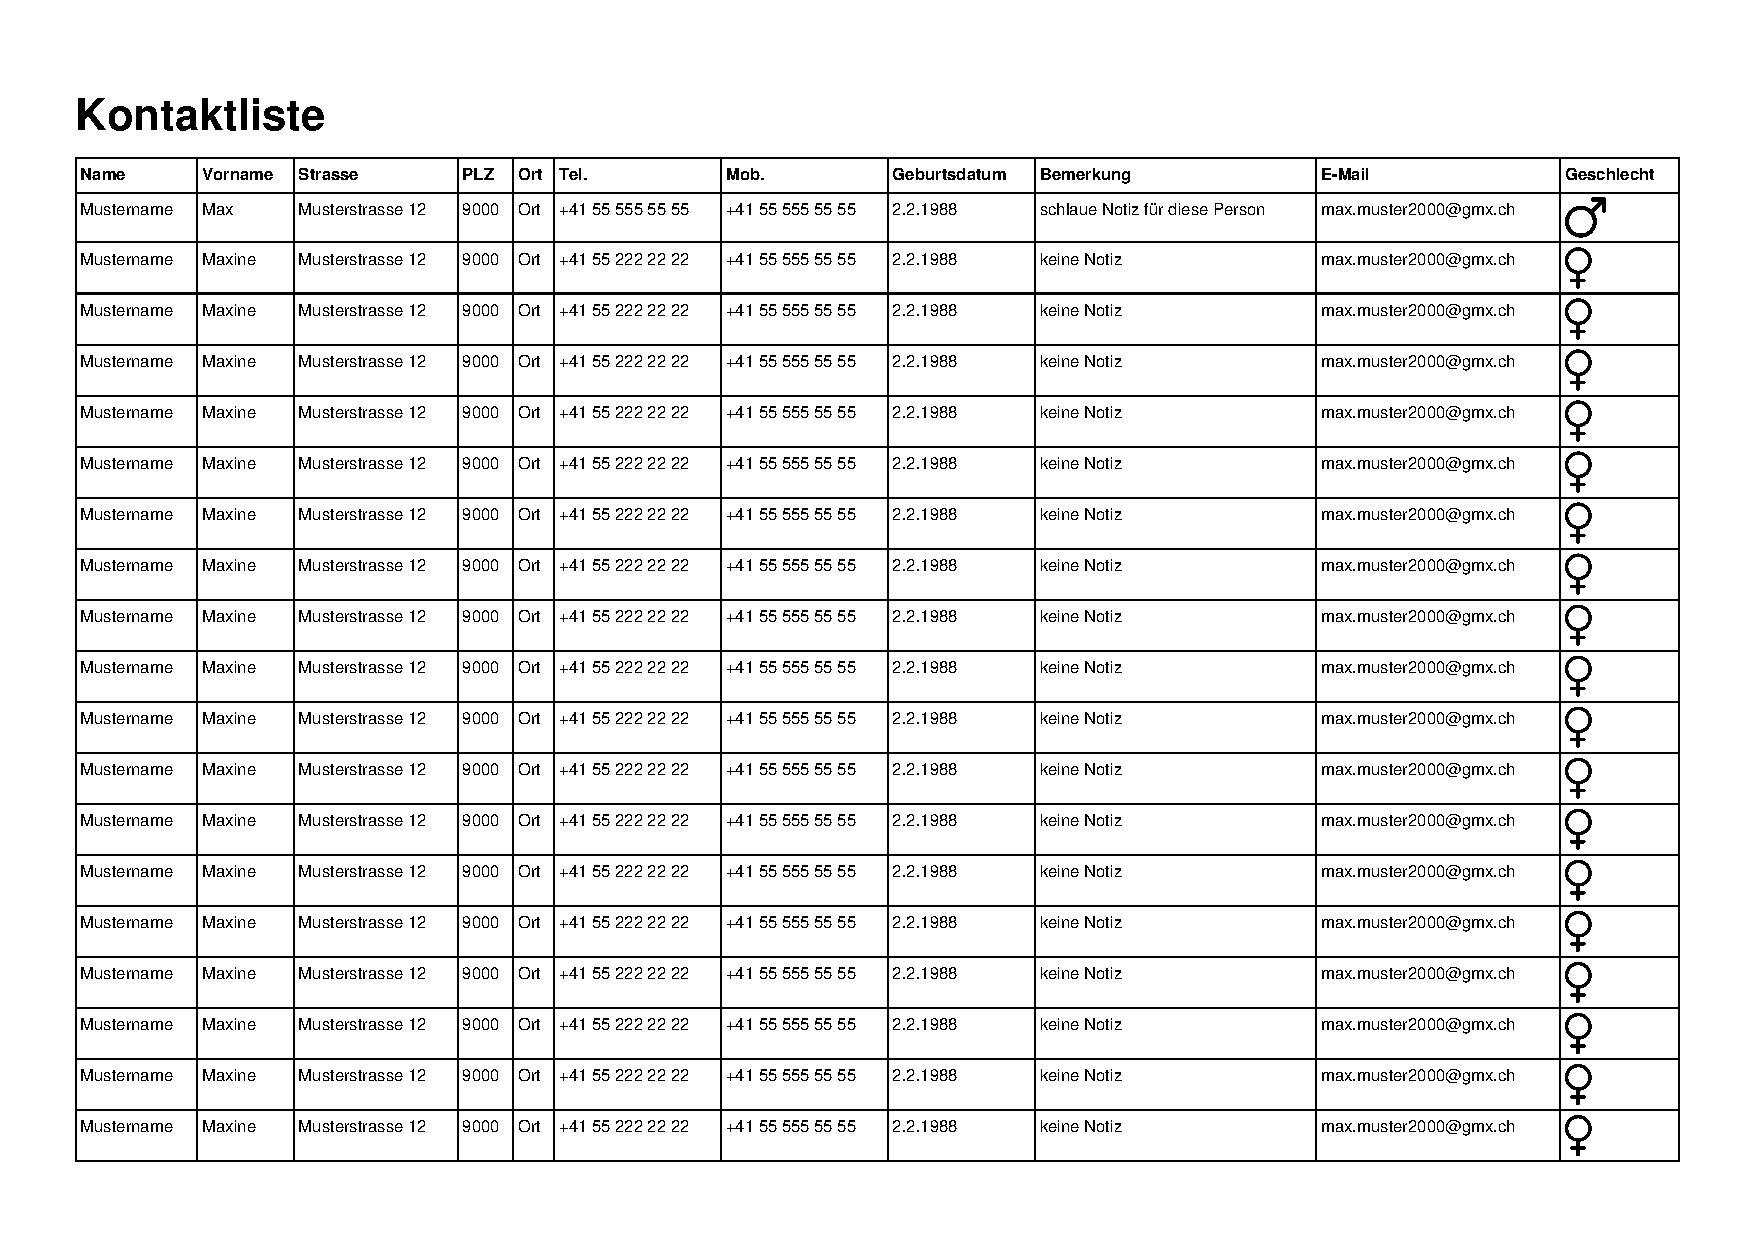
\includegraphics[scale=0.16]{mainpart/3_methodik_evaluation_img/itextSZ3.pdf}}

In diesem Anwendungsfall soll gezeigt werden welche  OSRE für z.B. einem Rechnungslauf am besten geeignet wäre. Dieser Anwendungsfall generiert zwar nur Reports die ein bis zwei Seiten lang sind aber diese müssen meisst über die Zeitspanne einer Nacht erstellt werden können. 



\section{Konsolidierung}
In diesem Schritt der Evaluation geht es darum die Daten zu vereinheitlichen und zu konsolidieren.

\textbf{Log Datei}

Aus den Daten die Heroku nieder schreibt sind unter anderem die eingehenden Requests, den Dyno Load und den Memoryverbrauch. Diese Daten werden als Zeichenketten in die Loggs geschrieben das aber nicht gesteuert von den Aktivitäten auf dem Dyno, sondern aufgrund eines Timers werden diese Daten aus einer Probe der Dyno gelesen und in die Logs persistiert. Um diese Daten auswerten zu können wurde einen eigenen Log Parser geschrieben, mit welchem es möglich ist die diese Logs zu finden und in eigenen kommaseparierten Daten zu speichern.   

\begin{reference}{Log Extractor Source Code}
Den Log Extractor kann hier gefunden werden:  \url{https://github.com/denisbittante/dinf/tree/master/loadtest/utils/src/ch/ffhs/dinf/utils/log}
 
\end{reference}



\textbf{JMeter Testresultate}


Die Ergebnisse können wiederum mit JMeter im Gui-Modus gelesen und ausgewertet werden. 



\begin{reference}{Konsolidierten Daten}
Die Konsolidierten Daten können hier heruntergeladen werden:  \url{https://github.com/denisbittante/dinf/tree/master/loadtest/results}
 
\end{reference}









\end{document}